\subsection{Architettura generale - Componenti del sistema}
\subsubsection{Monolith}
   \FloatBarrier
   \begin{figure}[ht]
   \centering
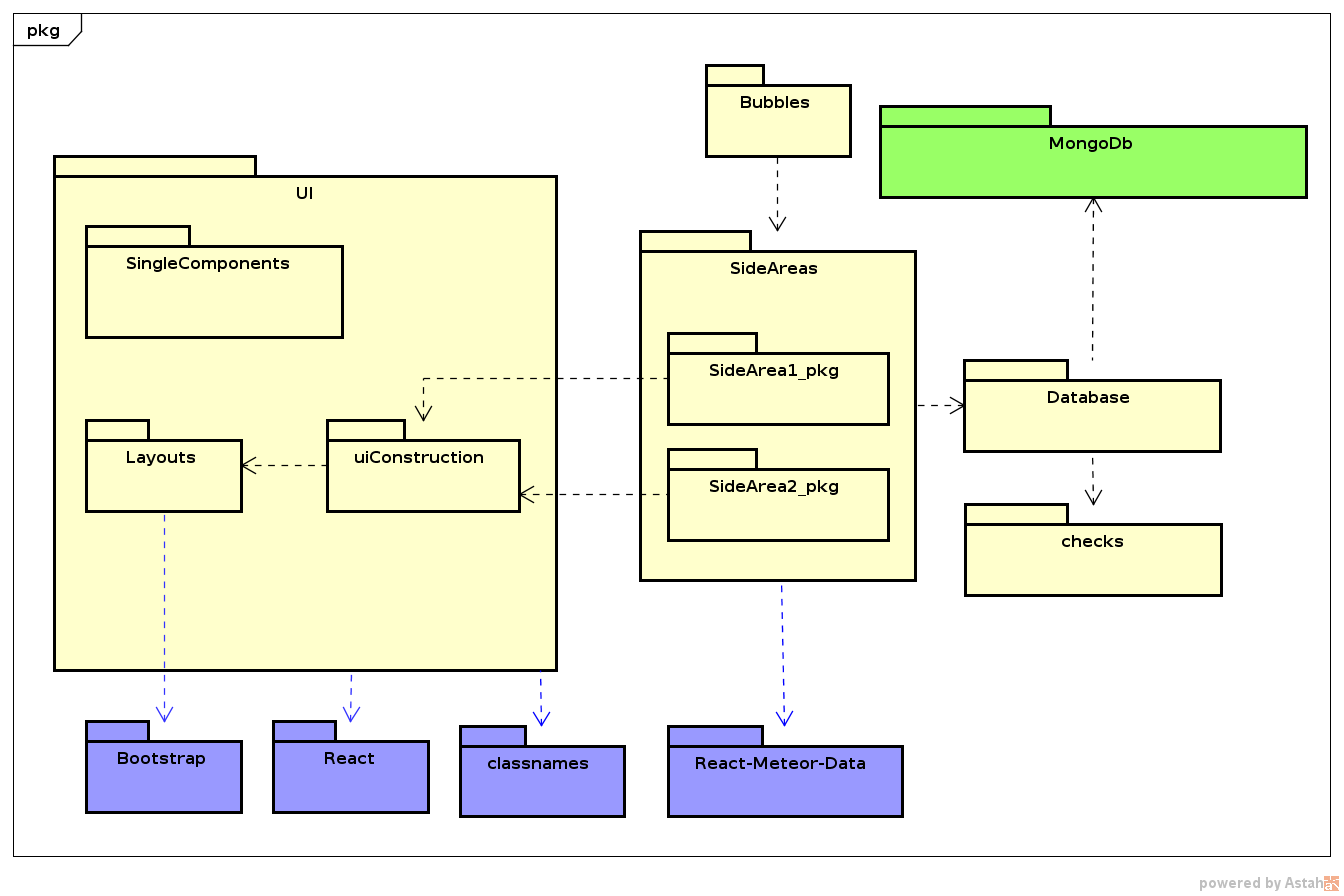
\includegraphics[width=\textwidth,keepaspectratio]{img/General}
   \caption{Diagramma per Monolith.}
\end{figure}
\FloatBarrier
\textbf{Descrizione}:\\
 Componente che rappresenta l'intera SDK di Monolith 


\clearpage

\subsubsection{Monolith::Bubbles}
   \FloatBarrier
   \begin{figure}[ht]
   \centering
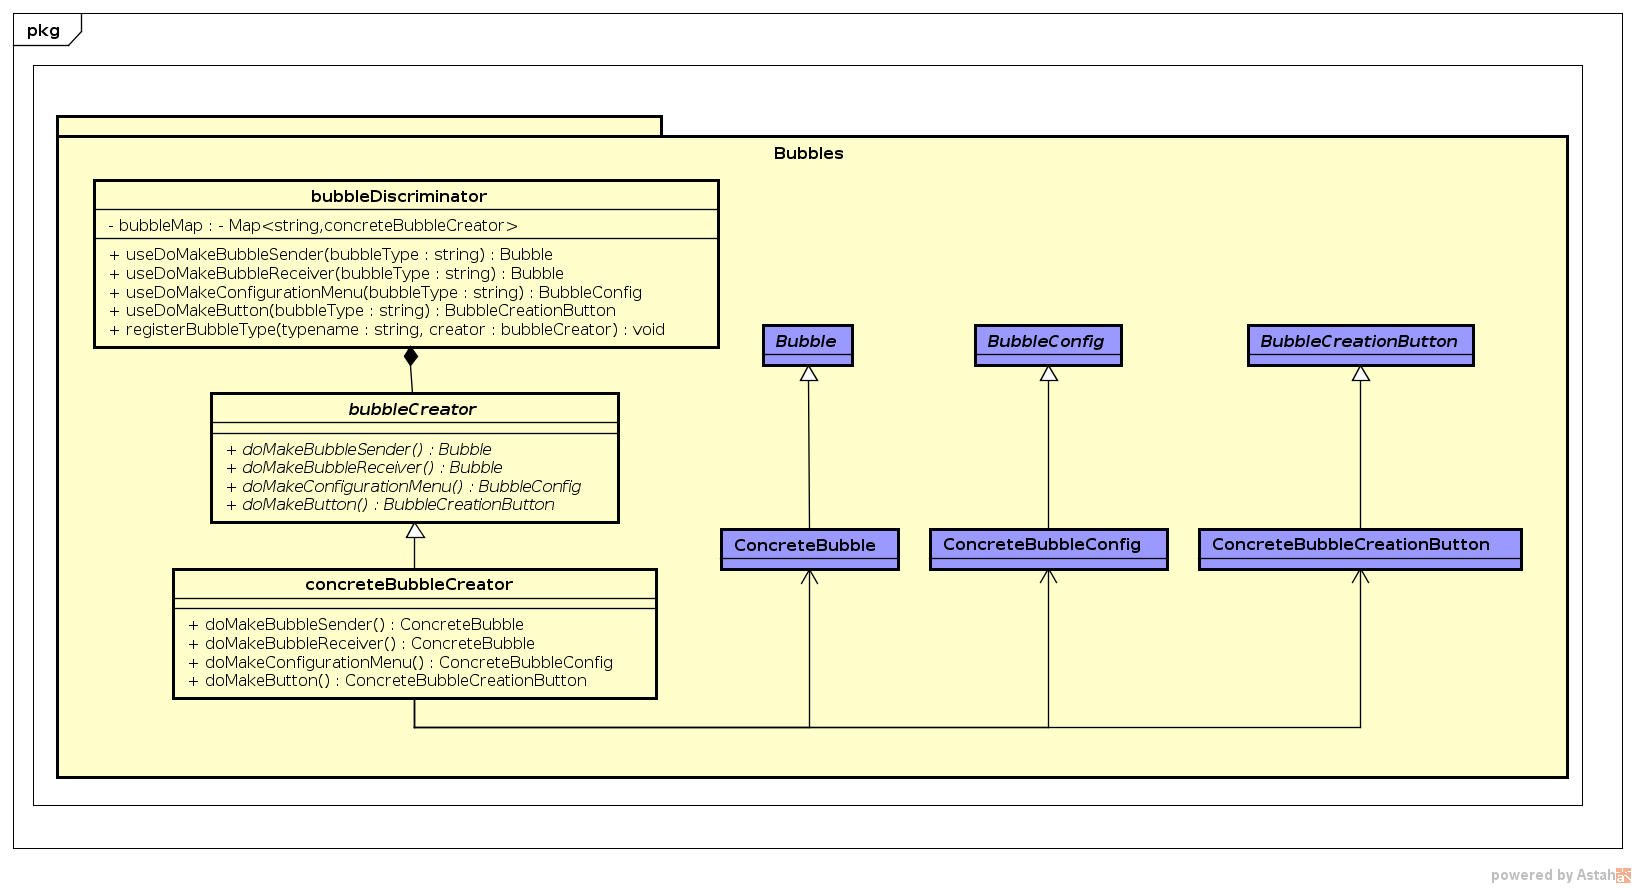
\includegraphics[width=\textwidth,keepaspectratio]{img/Bubbles}
   \caption{Diagramma per Monolith::Bubbles.}
\end{figure}
\FloatBarrier
\textbf{Descrizione}:\\
 Componente che contiene i pacchetti delle bolle predefinite include in Monolith 


\clearpage

\subsubsection{Monolith::checks}
   \FloatBarrier
   \begin{figure}[ht]
   \centering
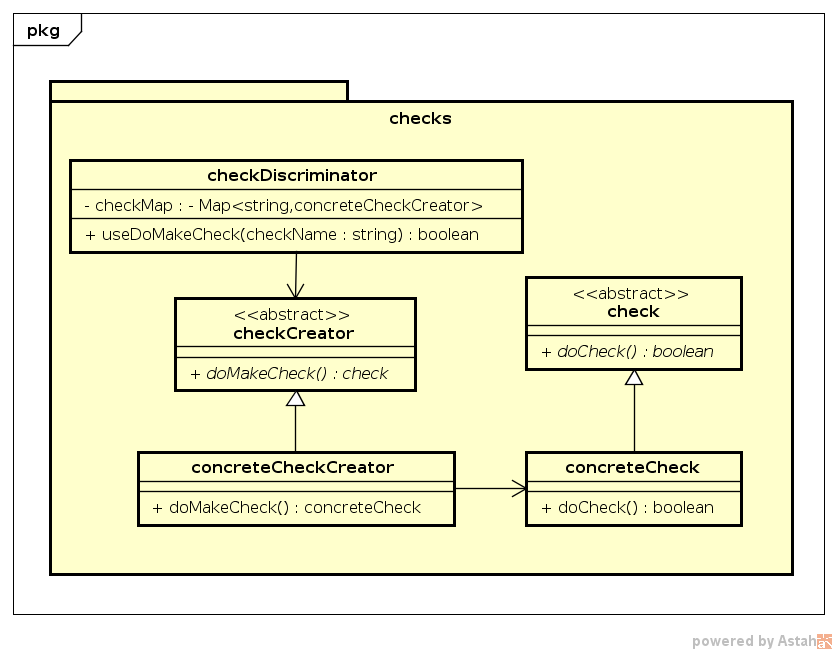
\includegraphics[width=\textwidth,keepaspectratio]{img/controls}
   \caption{Diagramma per Monolith::checks.}
\end{figure}
\FloatBarrier
\textbf{Descrizione}:\\
 Componente che contiene il codice necessario a eseguire controlli sugli input degli utenti. Dipende dalla libreria SimpleSchema. 
\\ \textbf{Classi contenute}:\\
\begin{itemize}
\item Check
\item CheckHandler
\end{itemize}


\clearpage

\subsubsection{Monolith::Database}
   \FloatBarrier
   \begin{figure}[ht]
   \centering
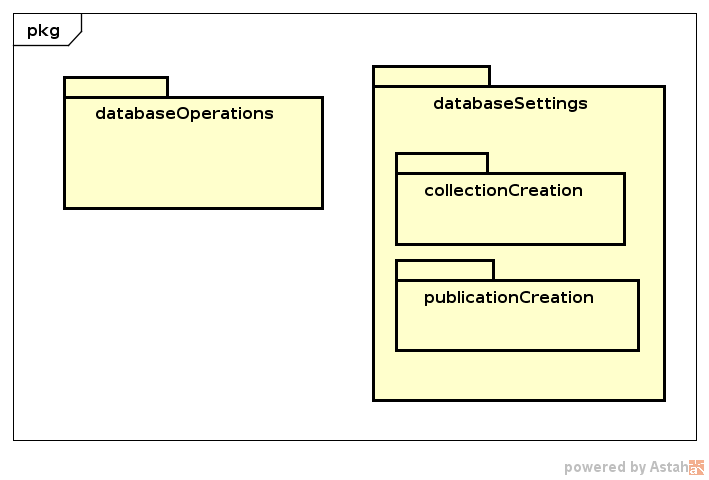
\includegraphics[width=\textwidth,keepaspectratio]{img/database}
   \caption{Diagramma per Monolith::Database.}
\end{figure}
\FloatBarrier
\textbf{Descrizione}:\\
 Componente contenente i pacchetti che vengono utilizzati per interagire con il database 
\\ \textbf{Classi contenute}:\\
\begin{itemize}
\item BubbleDatabase
\end{itemize}


\clearpage

\subsubsection{Monolith::Database::databaseInitialization}
\textbf{Descrizione}:\\
 Componente che si occupa di inizializzare e esportare la collezione che memorizza le bolle e di effettuare la pubblicazione (Meteor.Publish). Viene fornita anche una versione della collezione da utilizzare con il meccanismo delle promises grazie alla libreria Bluebird. 


\clearpage

\subsubsection{Monolith::Database::Methods}
\textbf{Descrizione}:\\
 Componente che contiene i principali Meteor.Methods  che riguardano le bolle:
\\begin{itemize}
\\item insertBubble(bubbleType, roomId, data, funDataEdit, funDataEditArgs) \\\\
Effettua i controlli sull'input tramite il pacchetto Monolith::checks. Aggiunge i dati che devono essere presenti in ogni bolla (indipendentemente dal tipo) e in caso di successo l'operazione viene eseguita sul database.\\\\
Gli ultimi due argomenti sono opzionali e sono il nome di un Meteor.Method e i suoi eventuali argomenti. In caso tale argomento sia presente il metodo indicato viene usato sull'oggetto data prima di effettuare i controlli. In questo modo è possibile stabilire operazioni da svolgere lato server.
\\item updateBubble(bubbleId, funDataEdit, funDataEditArgs)\\\\
\\item removeBubble(bubbleId) \\\\
La bolla con l'id passato come argomento viene eliminata dal database,
\\end{itemize} 


\clearpage

\subsubsection{Monolith::SideAreas}
\textbf{Descrizione}:\\
 Contiene i package per la visualizzazione delle bolle nelle side-bar 


\clearpage

\subsubsection{Monolith::SideAreas::SideArea1\_pkg}
   \FloatBarrier
   \begin{figure}[ht]
   \centering
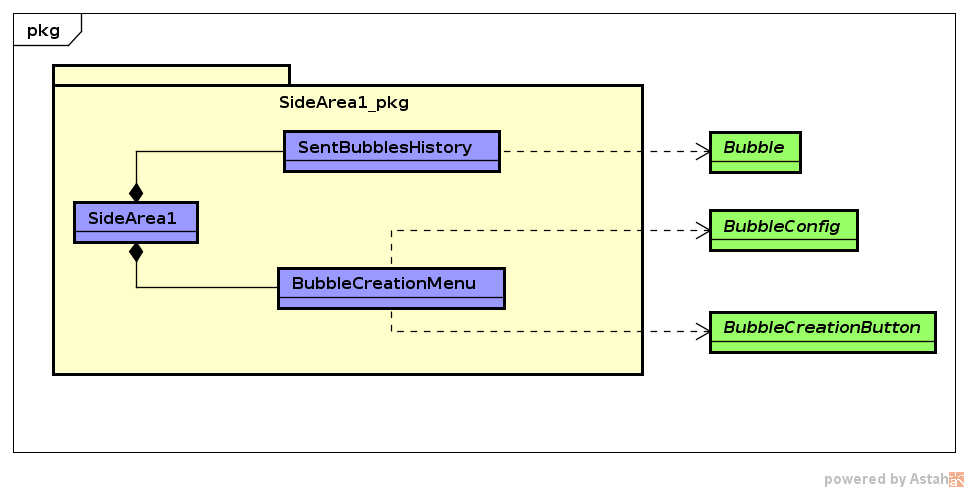
\includegraphics[width=\textwidth,keepaspectratio]{img/sd1_pkg}
   \caption{Diagramma per Monolith::SideAreas::SideArea1\_pkg.}
\end{figure}
\FloatBarrier
\textbf{Descrizione}:\\
 Componente per la visualizzazione delle bolle inviate e del menù di creazione delle bolle nella prima side area 
\\ \textbf{Classi contenute}:\\
\begin{itemize}
\item BubbleMenu
\item ConfigArea
\item SentBubbles
\item SideArea1
\end{itemize}


\clearpage

\subsubsection{Monolith::SideAreas::SideArea2\_pkg}
   \FloatBarrier
   \begin{figure}[ht]
   \centering
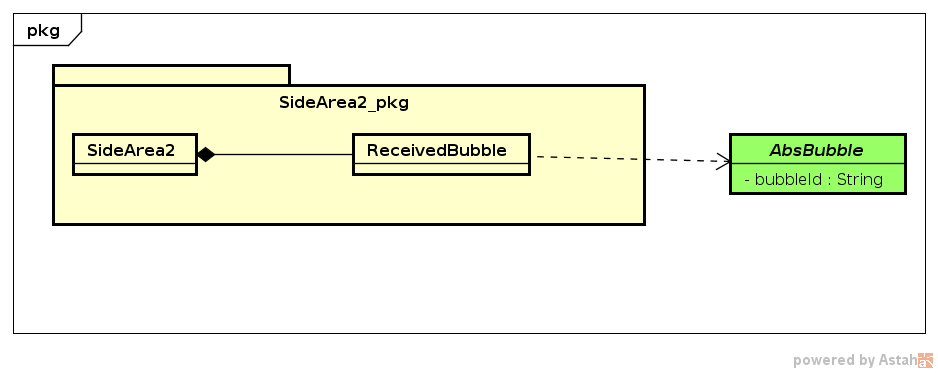
\includegraphics[width=\textwidth,keepaspectratio]{img/sd2_pkg}
   \caption{Diagramma per Monolith::SideAreas::SideArea2\_pkg.}
\end{figure}
\FloatBarrier
\textbf{Descrizione}:\\
 Componente per la visualizzazione delle bolle ricevute nella seconda side area 
\\ \textbf{Classi contenute}:\\
\begin{itemize}
\item ReceivedBubble
\item SideArea2
\end{itemize}


\clearpage

\subsubsection{Monolith::UI}
\textbf{Descrizione}:\\
 Componente contenente tutti i pacchetti che servono per comporre e gestire la parte visuale dell'applicazione delle bolle \\\\
\\textbf{Dipendenze}
\\begin{itemize}
\\item React
\\item classNames
\\end{itemize} 


\clearpage

\subsubsection{Monolith::UI::Layouts}
   \FloatBarrier
   \begin{figure}[ht]
   \centering
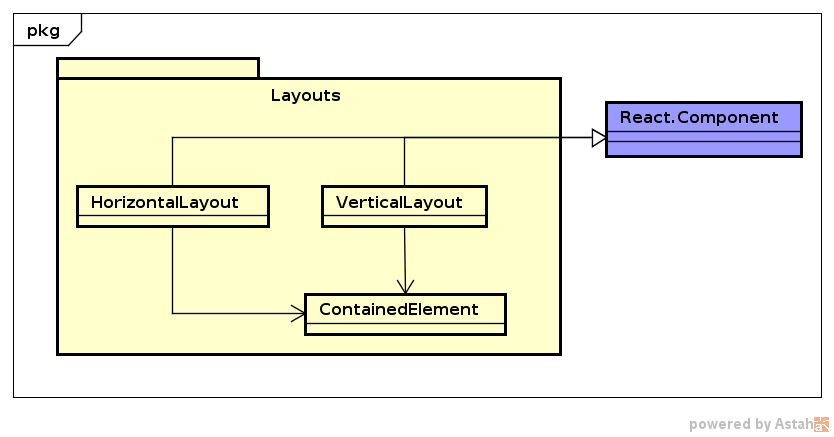
\includegraphics[width=\textwidth,keepaspectratio]{img/UI-Layouts}
   \caption{Diagramma per Monolith::UI::Layouts.}
\end{figure}
\FloatBarrier
\textbf{Descrizione}:\\
 Componente che contiene le classi React per la gestione dei layout \\\\
\textbf{Dipendenze} \\
Bootstrap 
\\ \textbf{Classi contenute}:\\
\begin{itemize}
\item ContainedElement
\item HorizontalLayout
\item VerticalLayout
\end{itemize}


\clearpage

\subsubsection{Monolith::UI::SingleComponents}
   \FloatBarrier
   \begin{figure}[ht]
   \centering
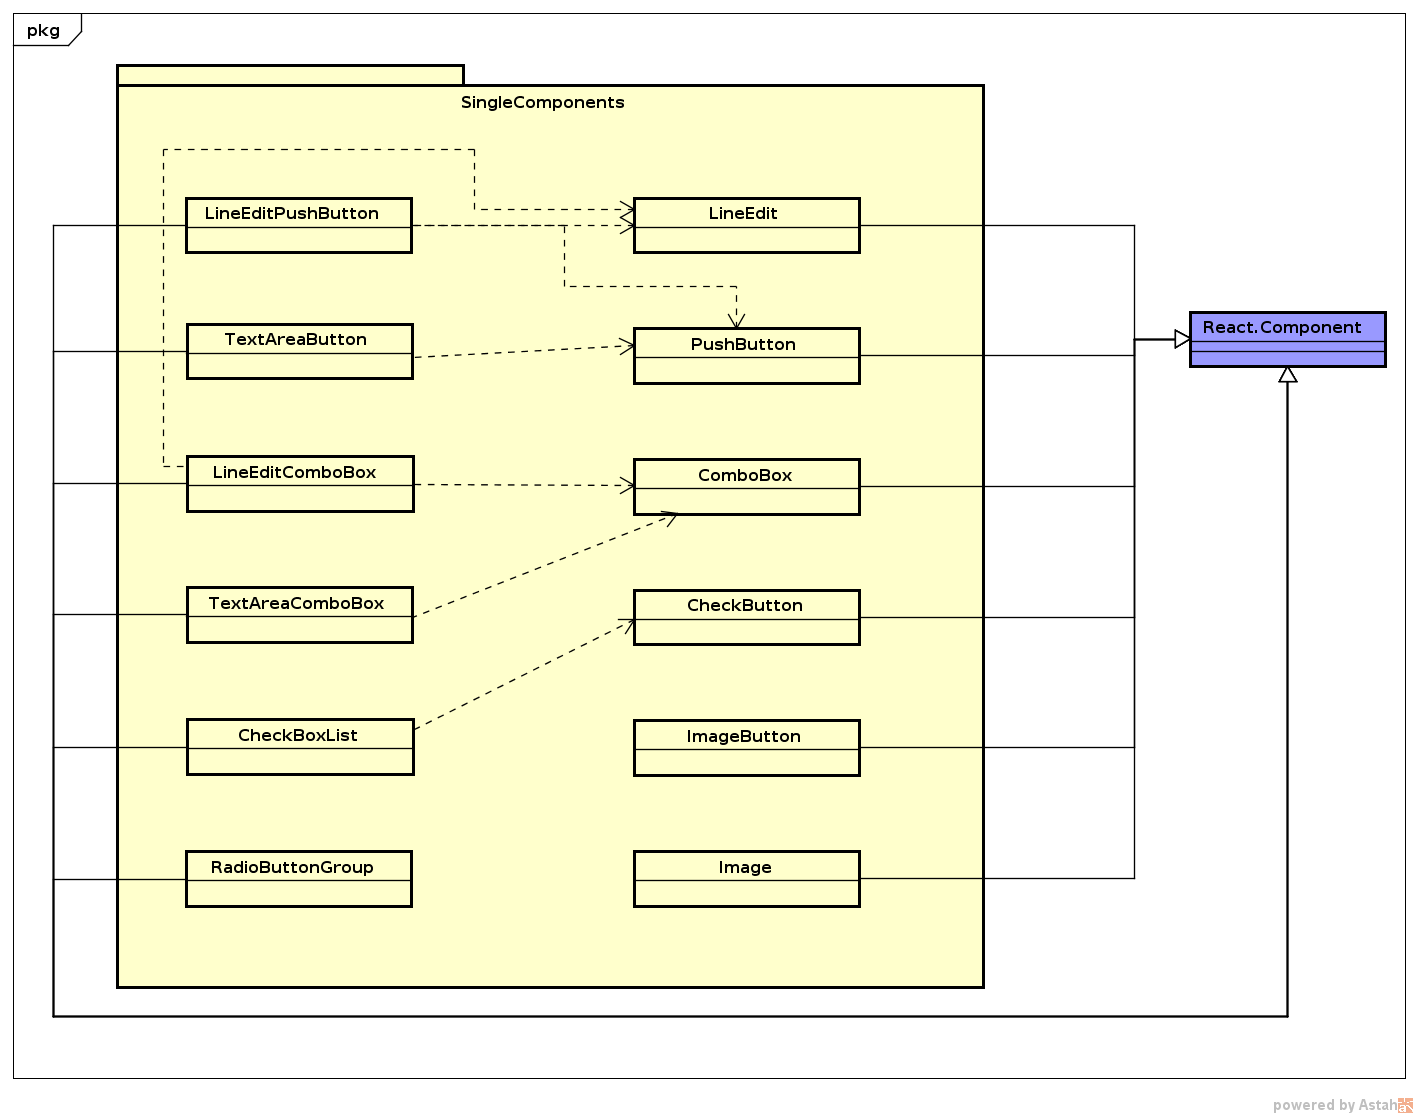
\includegraphics[width=\textwidth,keepaspectratio]{img/UI-SingleComponents}
   \caption{Diagramma per Monolith::UI::SingleComponents.}
\end{figure}
\FloatBarrier
\textbf{Descrizione}:\\
 Componente che contiene tutti i componenti React per la composizione della GUI 
\\ \textbf{Classi contenute}:\\
\begin{itemize}
\item CheckBoxList
\item CheckButton
\item ComboBox
\item Image
\item ImageButton
\item LineEdit
\item LineEditComboBox
\item LineEditPushButton
\item PushButton
\item RadioButtonGroup
\item TextAreaButton
\item TextAreaComboBox
\end{itemize}


\clearpage

\subsubsection{Monolith::UI::uiConstruction}
   \FloatBarrier
 %  \begin{sidewaysfigure}[ht]
%\begin{center}
 \makebox[\textwidth][c]{
\rotatebox{90}{
% \centering
\begin{minipage}{0.8\textheight}
   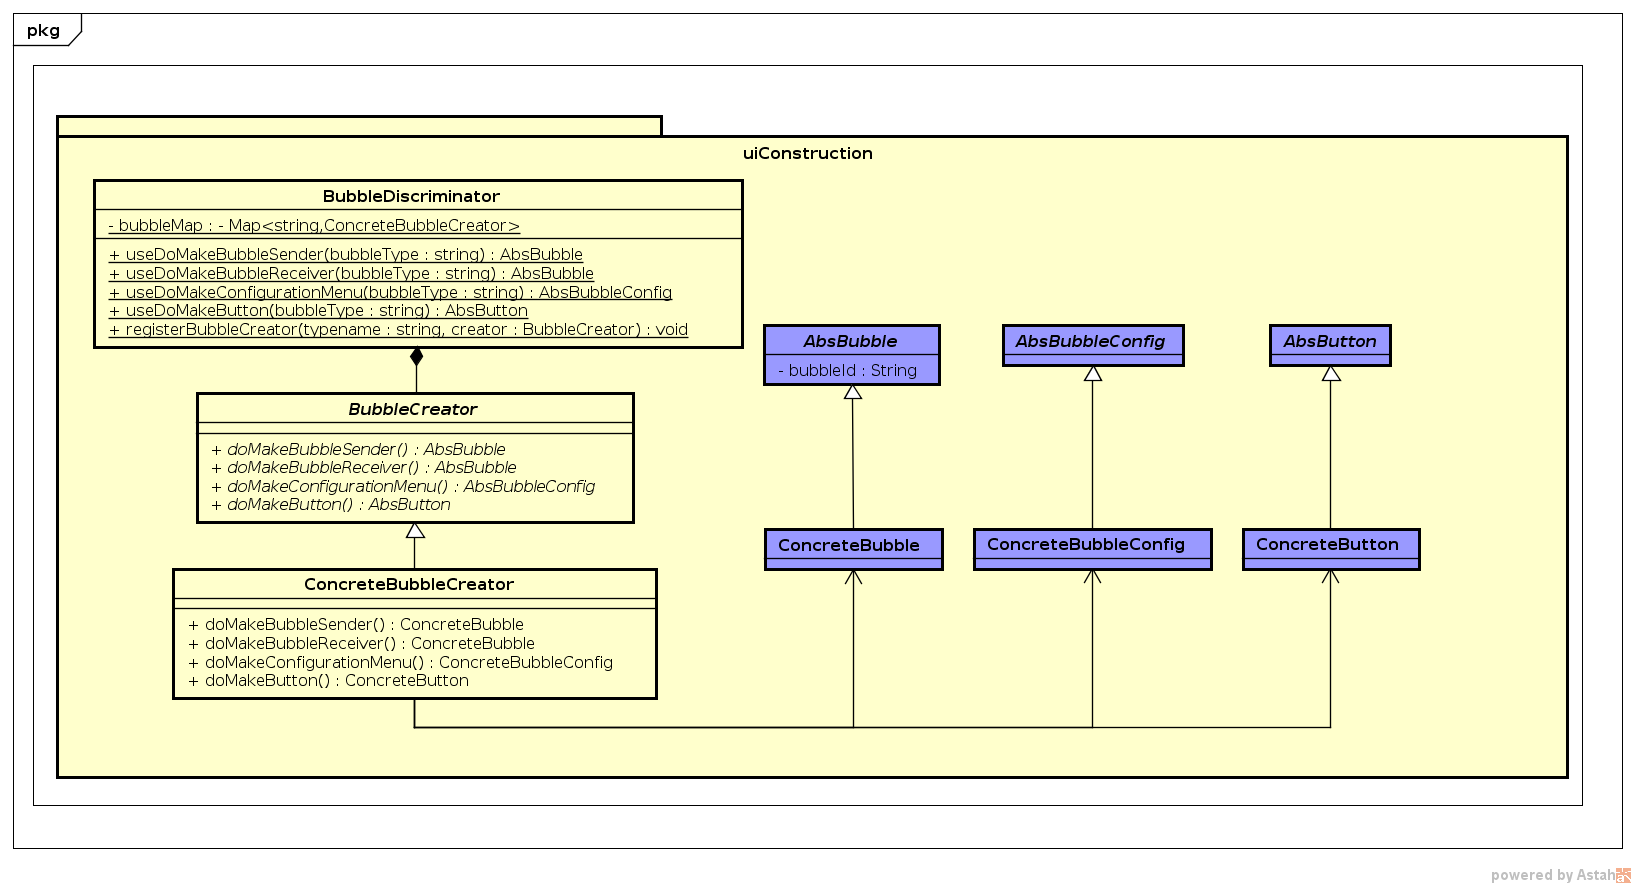
\includegraphics[width=\textwidth,keepaspectratio]{img/uiConstr}
  \captionof{figure}{Diagramma per Monolith::UI::uiConstruction.}
\end{minipage}}
}
%\end{center}
%\end{sidewaysfigure}
\FloatBarrier
\textbf{Descrizione}:\\
 Componente per la creazione delle bolle da visualizzare 
\\ \textbf{Classi contenute}:\\
\begin{itemize}
\item AbsBubble
\item AbsBubbleConfig
\item AbsButton
\item bubbleCreator
\item bubbleDiscriminator
\end{itemize}


\clearpage \subsection{Architettura generale - Bolle Demo}
\subsubsection{CurrencyBubble}
   \FloatBarrier
 %  \begin{sidewaysfigure}[ht]
%\begin{center}
 \makebox[\textwidth][c]{
\rotatebox{90}{
% \centering
\begin{minipage}{0.8\textheight}
   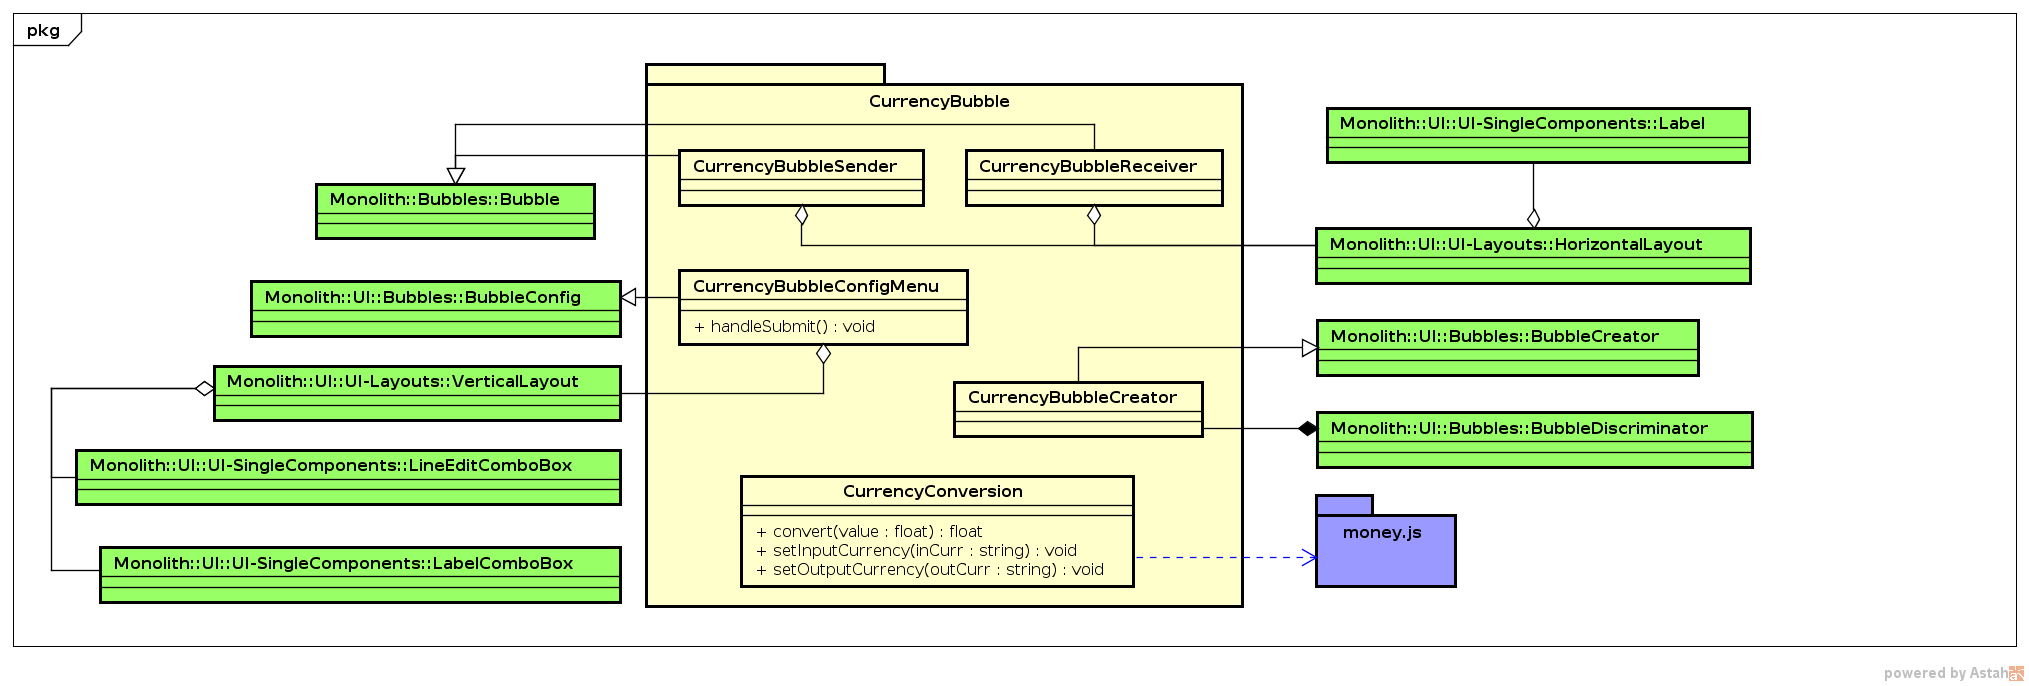
\includegraphics[width=\textwidth,keepaspectratio]{img/currency}
  \captionof{figure}{Diagramma per CurrencyBubble.}
\end{minipage}}
}
%\end{center}
%\end{sidewaysfigure}
\FloatBarrier
\textbf{Descrizione}:\\
 Componente contente le classi necessarie per la creazione della bolla convertitore valute. 
\\ \textbf{Classi contenute}:\\
\begin{itemize}
\item CurrencyBubble
\item CurrencyBubbleConfig
\item CurrencyBubbleCreationButton
\item CurrencyCreator
\end{itemize}


\clearpage

\subsubsection{CurrencyBubble::CurrencyMethod}
\textbf{Descrizione}:\\
 Componente che contiene la definizione dei Meteor.methods per le operazioni lato server della bolla currency.  In particolare BubbleCurrencyConvertor viene invocato dal metodo di inserimento di una nuova bolla per eseguire la conversione di valuta modificando l'oggetto inviato dal client prima dell'inserimento nel database. Utilizza la libreria request per scaricare da openexchangerates.org i dati di cui ha bisogno. Poi utilizza money.js per effettuare la conversione vera e propria. Ritorna poi l'oggetto modificato, pronto per essere inserito nel database. 


\clearpage

\subsubsection{ListBubble}
\textbf{Descrizione}:\\
 Componente contenente i pacchetti necessari per la creazione della bolla lista. 


\clearpage

\subsubsection{ListBubble::CheckListCreation}
\textbf{Descrizione}:\\
 Componente che si occupa della creazione delle check list. 
\\ \textbf{Classi contenute}:\\
\begin{itemize}
\item ListBubbleConfig
\item ListBubbleCreationButton
\end{itemize}


\clearpage

\subsubsection{ListBubble::CheckListReading}
\textbf{Descrizione}:\\
 Componente che si occupa della lettura e dell'utilizzo delle check list. 
\\ \textbf{Classi contenute}:\\
\begin{itemize}
\item ListBubble
\end{itemize}


\clearpage

\subsubsection{ListBubble::Configuration}
\textbf{Descrizione}:\\
 Componente che gestisce l'area di configurazione della bolla e il pulsante apposito da inserire nel menu iniziale di creazione. 


\clearpage

\subsubsection{ListBubble::DataManagement}
\textbf{Descrizione}:\\
 Componente che si occupa di tutte le operazioni di gestione dei dati che non sono gestite da Monolith. Usa il database MongoDB. 
\\ \textbf{Classi contenute}:\\
\begin{itemize}
\item ListBubbleCreator
\end{itemize}


\clearpage

\subsubsection{ListBubble::Receiver}
\textbf{Descrizione}:\\
 Componente che gestisce la visualizzazione della bolla da parte del ricevente. 


\clearpage

\subsubsection{ListBubble::Sender}
\textbf{Descrizione}:\\
 Componente che gestisce la visualizzazione della bolla da parte del mittente. 


\clearpage

\subsubsection{PollBubble}
   \FloatBarrier
 %  \begin{sidewaysfigure}[ht]
%\begin{center}
 \makebox[\textwidth][c]{
\rotatebox{90}{
% \centering
\begin{minipage}{0.8\textheight}
   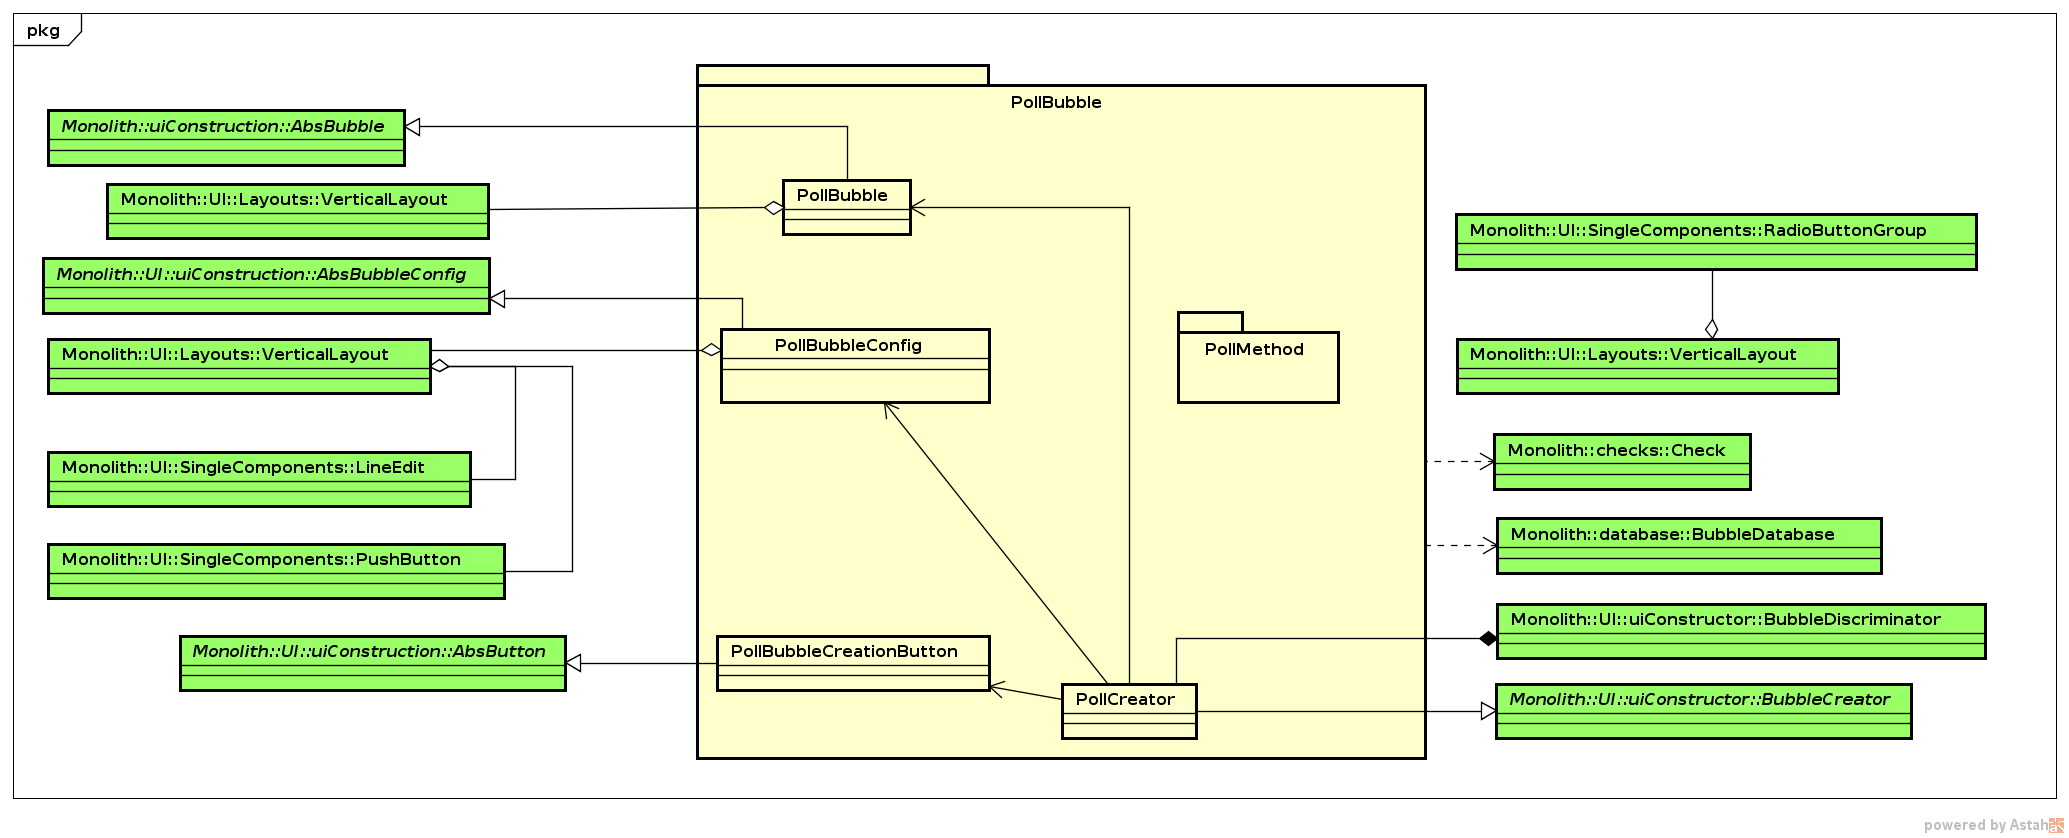
\includegraphics[width=\textwidth,keepaspectratio]{img/poll}
  \captionof{figure}{Diagramma per PollBubble.}
\end{minipage}}
}
%\end{center}
%\end{sidewaysfigure}
\FloatBarrier
\textbf{Descrizione}:\\
 Componente contente le classi necessarie per la creazione della bolla sondaggio. 
\\ \textbf{Classi contenute}:\\
\begin{itemize}
\item PollBubble
\item PollBubbleConfig
\item PollBubbleCreationButton
\item PollCreator
\end{itemize}


\clearpage

\subsubsection{PollBubble::PollMethod}
\textbf{Descrizione}:\\
 Componente che contiene la definizione dei Meteor.methods per le operazioni lato server della bolla poll,  In particolare BubblePollUpdate viene invocato dal metodo di aggiornamento di una bolla per incrementare il contatore dei voti. Utilizza direttamente l'accesso alla collezione su MongoDb 


\clearpage

\subsubsection{RandomBubble}
   \FloatBarrier
 %  \begin{sidewaysfigure}[ht]
%\begin{center}
 \makebox[\textwidth][c]{
\rotatebox{90}{
% \centering
\begin{minipage}{0.8\textheight}
   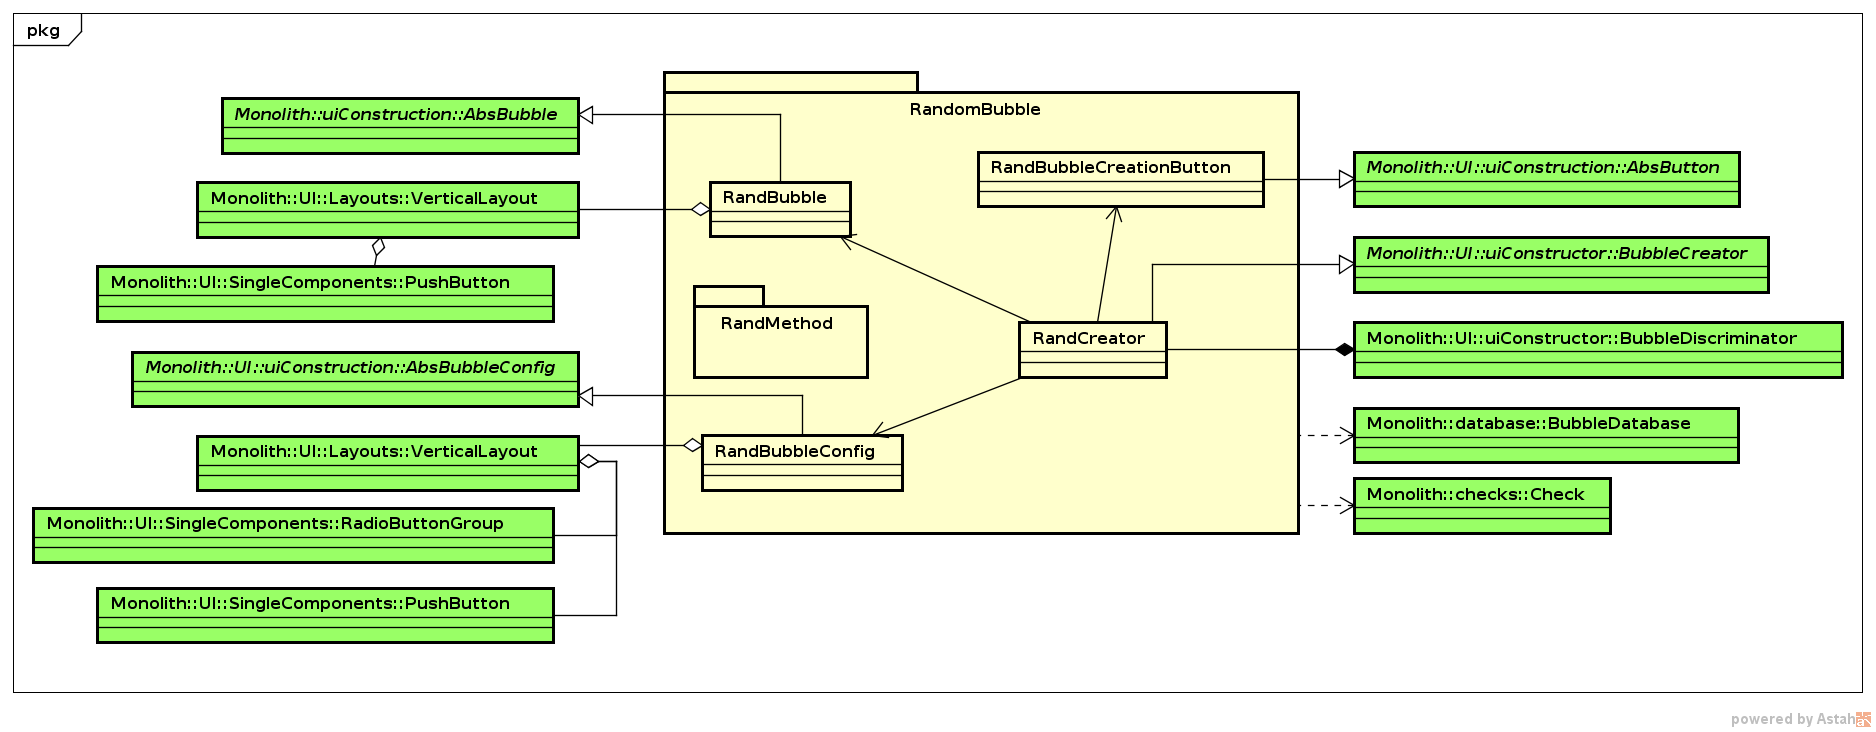
\includegraphics[width=\textwidth,keepaspectratio]{img/random}
  \captionof{figure}{Diagramma per RandomBubble.}
\end{minipage}}
}
%\end{center}
%\end{sidewaysfigure}
\FloatBarrier
\textbf{Descrizione}:\\
 Componente contente le classi necessarie per la creazione della bolla estrazione numero casuale. 
\\ \textbf{Classi contenute}:\\
\begin{itemize}
\item RandBubble
\item RandBubbleConfig
\item RandBubbleCreationButton
\item RandCreator
\end{itemize}


\clearpage

\subsubsection{RandomBubble::RandMethod}
\textbf{Descrizione}:\\
 Componente che contiene la definizione dei Meteor.methods per le operazioni lato server della bolla random.  In particolare:
\\begin{itemize}
\\item BubbleRandomInsert viene invocato dal metodo di inserimento di una nuova bolla per eseguire l'estrazione del numero casuale da inserire nel database.
\\item  BubbleRandomUpdate effettua un'operazione analoga a quella di BubbleRandomInsert ma per le operazioni di update.
\\end{itemize} 


